\section{Labelled triangular diagrams}
\label{sec:diagrams}

We next construct a two-dimensional labelled complex from the presentation
of $T$.  The presentation and link are the case $m=n=p=3$ of the
construction of Brady and McCammond \cite{BradyMcCammond2000}.
We give direct proofs of the needed facts.  This complex is separate
from the unknown CAT(0) space; the argument here concerns finite
diagrams and planar topology.

We need two conclusions.  Proposition~\ref{prop:sphere-counts} will
show that a spherical diagram has zero total signed occurrences of
each individual target triangle.  Lemma~\ref{lem:controlled-diagrams}
will approximate any geometric sphere map by a diagram, with one
distance bound valid on every point of every parameter triangle.
Together they will let the local winding count in
Section~\ref{sec:localization} use the metric separation from the
preceding section.

\subsection{The triangular presentation and its link}

\begin{lemma}\label{lem:triangular-presentation}
For each $(u,v)\in\mathcal E$, introduce two private generators
$x_{uv}$ and $h_{uv}$.  Write
$(x_1,x_2,x_3,h)=(u,v,x_{uv},h_{uv})$ within this block.  A presentation
of $T$ is given by the three relations
\begin{equation}\label{eq:triangle-relations}
  x_i x_{i+1}=h\qquad (i=1,2,3),
\end{equation}
in each block, where the subscripts on the $x_i$ are read modulo three.
\end{lemma}

\begin{proof}
The first two relations give $h=x_1x_2$ and
$x_3=x_2^{-1}x_1x_2$.  Substituting these in the third gives
$x_1x_2x_1=x_2x_1x_2$.  Conversely, that braid relation and these
definitions of $x_3,h$ give all three relations
\eqref{eq:triangle-relations}.  Since the added generators are private
to their blocks, eliminating them independently recovers the defining
presentation of $T$.
\end{proof}

Let $\mathcal A$ be the resulting set of nine generators.  Define the
labelled Cayley complex $\mathcal K$ as follows.  Its vertices are the
elements of $T$.  For every $g\in T$ and $q\in\mathcal A$ there is an
oriented edge labelled $(g,q)$ from $g$ to $gq$.  For each relation
\eqref{eq:triangle-relations} and each $g$, attach a triangle, with its
own cell identity, along the edges joining
\begin{equation}\label{eq:triangle-vertices}
  g,\quad gx_i,\quad gh.
\end{equation}
Edges and triangles retain these identities even if some other cells
have the same vertex data.  The homomorphism $T\to\mathbb Z$ taking
$a,b,c$ to $1$ takes every $x_i$ to $1$ and every $h$ to $2$.
Consequently the three vertices in \eqref{eq:triangle-vertices} are
distinct.  In particular every target triangle has three distinct
sides and three distinct corners.

The link at a vertex means the graph with one vertex for each incident
edge direction and one edge for each incident triangle corner.  Its
vertices can be denoted $q^+,q^-$ for $q\in\mathcal A$, representing
the outgoing and incoming $q$-edges.

\begin{lemma}\label{lem:link-girth}
The link at every vertex of $\mathcal K$ has no circuit of length
less than six, including circuits formed by parallel edges.
\end{lemma}

\begin{proof}
Fix a Cayley vertex $v$.  For the relation $x_ix_{i+1}=h$, its
initial, middle, and terminal corners occur at $v$ in exactly the
translates
$g=v$, $g=vx_i^{-1}$, and $g=vh^{-1}$, respectively.  Their link
edges are exactly
\begin{equation}\label{eq:link-edges}
  \{x_i^+,h^+\},\qquad
  \{x_i^-,x_{i+1}^+\},\qquad
  \{x_{i+1}^-,h^-\}.
\end{equation}
Thus one block is a theta graph with three internally disjoint paths
of length three from $h^+$ to $h^-$:
\[
 \begin{gathered}
 h^+\; -\; x_1^+\; -\; x_3^-\; -\; h^-,\\
 h^+\; -\; x_2^+\; -\; x_1^-\; -\; h^-,\\
 h^+\; -\; x_3^+\; -\; x_2^-\; -\; h^-.
 \end{gathered}
\]
Its nine link edges are distinct.
The three blocks meet only at the signed directions of $a,b,c$.
Across different blocks the only link edges whose two endpoints are
shared directions are
\[
  \{a^-,b^+\},\qquad \{b^-,c^+\},\qquad \{c^-,a^+\}.
\]
They too are distinct.  This verifies both the complete link
description and the absence of parallel edges; possible coincidences
of group elements do not identify labelled edge directions.

It remains to bound a simple circuit.  A circuit staying within one
block has length at least six.  Otherwise split it into maximal
nonempty paths within individual blocks, and let $k$ be their number.
Their endpoints are the places where the circuit changes blocks.
If $k=2$, both changes occur in the intersection of the same two
blocks.  Their endpoints must be the two distinct signs of the one
shared generator.  Within either block their distance is three, so
the circuit has length at least six.

If $k=3$, the circuit visits all three blocks, changing at one signed
direction of each of $a,b,c$.  In a block the two relevant directions
are those of $x_1,x_2$.  Equal signs have distance at least two;
opposite signs have distance at least three except for
$x_1^-,x_2^+$, which are adjacent.  When all three signs agree, the
length is therefore at least $2+2+2$.  Otherwise there are two
changes of sign in the cyclic order $a,b,c,a$: one from minus to
plus, and one from plus to minus.  At most one of the corresponding
two block paths can use the exceptional adjacency.  The lower bound
is then $1+3+2=6$.

Finally, if $k\ge4$, a block path of length one must be one of the
three displayed edges between shared directions.  Each shared
direction is incident to at most one such edge, so two length-one
paths cannot be consecutive on the simple circuit.  At most
$\lfloor k/2\rfloor$ paths have length one and the others have length
at least two.  The total length is at least
$2k-\lfloor k/2\rfloor\ge6$.
\end{proof}

\subsection{Signed counts on spheres}

A combinatorial map to $\mathcal K$ will always include cell identities.
Each edge maps to a specified target edge, possibly with its
orientation reversed, or to a vertex.  Each triangle either maps
homeomorphically to a specified target triangle by its vertex
correspondence, or maps affinely into a specified target edge or
vertex.  These choices agree on common sides.  We call the latter
triangles collapsed.  Fix an orientation for every target triangle.
On an oriented source surface, a noncollapsed triangle has sign
$+1$ or $-1$ according to its map to that oriented target.

The proof below uses the classical diagrammatic-reducibility method of
deleting opposite faces and excluding a reduced spherical diagram by
curvature \cite[Definition~3.1 and Corollary~4.6]{Gersten1987}, here
keeping the identity of each target cell and allowing collapsed parameter
triangles.

\begin{proposition}\label{prop:sphere-counts}
For every combinatorial map from a finite triangulated oriented
two-sphere to $\mathcal K$, and every individual target triangle
$\tau$, the sum of the signs of all occurrences of $\tau$ is zero.
Collapsed triangles are allowed in the map and contribute zero.
\end{proposition}

\begin{proof}
\textit{Encoding the sphere.}
In each noncollapsed source triangle draw a central node with three
legs ending at its side midpoints.  A triangle collapsed to an edge
has exactly two nonconstant sides.  Join their midpoints by an arc;
both sides map to the same labelled target edge.  A triangle
collapsed to a vertex needs no arc.  Joining across source sides
produces an embedded trivalent graph, together with possible closed
curves containing no nodes.  Discard these curves.  Each remaining
node records a particular occurrence of a target triangle, with
its orientation sign, and each graph edge pairs two sides mapping
to the same labelled target edge.

We must retain endpoint information before using this graph as a
diagram.  Give it a thin regular neighbourhood, consisting of node
disks and ribbons along the edges.  Along either side of a ribbon
the actual group label of the corresponding endpoint of its target
edge stays constant.  Indeed, passing through an edge-collapsed
triangle connects the two sides at the same endpoint of that
edge.  At a node the two ribbon sides bounding one sector carry
the same group label, namely the corresponding corner of that
target triangle.  It follows that every boundary circle of the
regular neighbourhood carries one group-vertex label throughout.

For each connected component containing nodes, cap its neighbourhood
by a disk on every boundary circle and use that constant label at
the corresponding dual vertex.  This gives a labelled triangular
cell decomposition of a sphere: graph nodes correspond to its
triangular faces, graph edges to its edges, and neighbourhood
boundary circles to its vertices.  Here we use the elementary finite
planar-topology fact that a polygonal arc properly embedded in a disk cuts it into two disks.
To see how it applies, thicken a spanning tree of the connected
planar graph to a disk.  Add the other embedded edges one at a time
as bands.
Each runs through a complementary disk and divides it into two
disks.  Capping the remaining boundary circles therefore gives a
sphere.  This also proves the usual Euler formula for the resulting
cell decomposition.  It need not be a strict simplicial complex;
incidences, rather than distinct pairs of vertices, are counted.

The labelling rules exclude certain possible degeneracies.  A
graph edge cannot join two legs at the same node: these legs
represent different target sides, whereas a ribbon has one fixed
target edge.  No two corners of a face can become the same dual
vertex, since their actual target vertex labels are distinct.
Also a bridge of the graph would have both ribbon sides on the
same neighbourhood boundary circle.  Constancy around that circle
would equate the distinct endpoints of its target edge, so a
correctly labelled graph here has no bridge.  Multiple edges
between different nodes are harmless.

\smallskip\noindent\textit{Deleting folds.}
A fold is a pair of faces sharing an edge and mapping to the same
target triangle across the same target side.  Their signs are
opposite.  Such a pair can be deleted directly in the planar
graph.  Take a small disk around the chosen connecting edge and
its two nodes, cutting the other four legs close to the nodes.
The chosen edge and its endpoint disks form a disk even if the
same two nodes have additional connecting edges: the middle
portions of those additional edges lie outside this disk.
If the remaining target sides are called $i,j$, the exposed legs
occur in cyclic order $i,j,j,i$, up to reversal and cyclic
permutation.  Join $i$ to $i$ and $j$ to $j$ inside the disk without
crossing and delete the two nodes.  The endpoint labels match on
each new ribbon side, including at the common target corner
between the two pairings.  This preserves all the label rules,
planarity, and the sum of signs for each target triangle.
It may separate components or produce circles without nodes;
discard such circles and cap the neighbourhoods of the remaining
components as above.
Figure~\ref{fig:fold} illustrates the reconnection and its endpoint labels.

\begin{figure}[htbp]
 \centering
 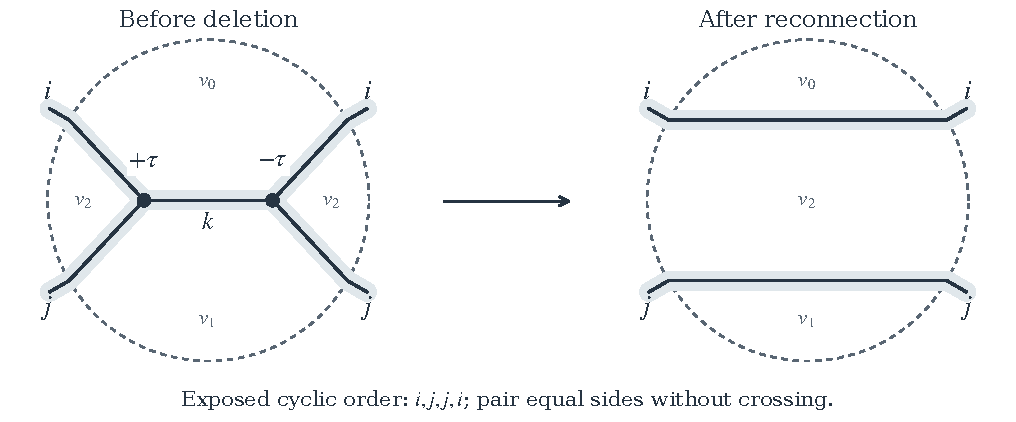
\includegraphics[width=\textwidth]{figures/fold.pdf}
 \caption{Deleting a fold.  The two nodes are oppositely signed
 occurrences of the same labelled target triangle \(\tau\), joined
 across side \(k\).  Its other sides are \(i,j\); the regions retain
 the actual vertex labels \(v_0,v_1,v_2\).
 Inside the dashed surgery disk, equal sides can be reconnected
 without crossing, preserving all endpoint labels.}
 \label{fig:fold}
\end{figure}

\smallskip\noindent\textit{The Euler contradiction.}
If nodes remain and no fold is available, choose a component and
its dual spherical cell decomposition.  The successive corners at
each dual vertex give a closed walk in the link of its actual
target vertex.  A backtrack in this walk would use the very same
target corner on both sides of a shared edge.  The exact corner
description \eqref{eq:link-edges} then identifies the same translated
target triangle on both sides, which is a fold.  These must be two
distinct source faces: one face cannot use two different corners
at this dual vertex, nor can two of its distinct sides be joined
by the same ribbon.  Thus a one-face incidence cannot evade the
deletion rule.

Every link walk is consequently nonbacktracking.  Any finite
nonempty closed nonbacktracking walk contains a circuit, so
Lemma~\ref{lem:link-girth} makes its length at least six.  Let
$F,E,V$ count faces, edges, and vertices of this dual component,
with all incidences counted.  We obtain
\[
  3F=2E,\qquad 2E\ge6V,\qquad V-E+F=2.
\]
The first two imply $V-E+F\le0$, a contradiction.  Thus whenever
nodes remain, a fold can be removed.  Each removal decreases their
number by two, so the process terminates with no nodes.  All
signed target-cell counts have been preserved and are then zero.
\end{proof}

\subsection{Controlled approximation by diagrams}

The next lemma transfers continuous maps into the geometric
$T$-space to diagrams.  A triangulation of a parameter surface
means a homeomorphism from a finite triangulated surface onto it.
Refinements below are performed within its existing faces, with
matching subdivisions of their boundaries.  In particular, a
prescribed subcomplex remains a union of closed triangles after
refinement; its underlying subset is never moved.

\begin{lemma}\label{lem:controlled-diagrams}
Suppose that $T$ acts geometrically on $Y$ and fix $y\in Y$.
There is a constant $C_1$, depending only on this action, $y$, and
the fixed presentation, with the following property.  Let $\Sigma$
be a triangulated parameter two-sphere, let $B$ be a subcomplex,
and let $f:\Sigma\to Y$ be continuous.  There is a refinement
keeping $B$ a subcomplex and a combinatorial map from the refined
sphere to $\mathcal K$ such that, for every final triangle $Q$,
every one of its group-vertex labels $s$, and every $p\in Q$,
\begin{equation}\label{eq:all-points-control}
  d_Y(sy,f(p))\le C_1.
\end{equation}
In particular $C_1$ is independent of $f$, its modulus of
continuity, and the number of triangles required.
\end{lemma}

\begin{proof}
\textit{Uniform boundary types.}
Choose $R<\infty$ such that every point of $Y$ is within $R$ of
$Ty$.  For example, if $Y=TK$ with $K$ compact, take
$R=\max_{z\in K}d_Y(y,z)$.  By Lemma~\ref{lem:orbit-control},
choose an integer $M$ such that
\begin{equation}\label{eq:bounded-edge-word}
  d_Y(sy,ty)\le2R+1\quad\Longrightarrow\quad d_T(s,t)\le M.
\end{equation}
Set
$D=\max\{d_Y(y,ay),d_Y(y,by),d_Y(y,cy)\}$.

By uniform continuity, first refine the given parameter
triangulation, still respecting $B$, until every face image has
diameter at most one.  Give each vertex $v$ a group label $s_v$
with $d_Y(s_vy,f(v))\le R$.  For each unoriented edge, choose once
and for all a path between its two labels of length at most $M$
in the Cayley graph on $a,b,c$; the opposite orientation uses
the reverse of this same path.  This is possible by
\eqref{eq:bounded-edge-word}.  Add three constant steps at each
end of every chosen path.  Subdivide the parameter edge
accordingly, once for both adjacent faces.  Its length is at
most $M+6$, and every face boundary is a labelled null loop
of length at most $3(M+6)$.

Relative to the label of an original vertex of a face, only
finitely many such boundary types are possible: their lengths
are bounded and their letters belong to
$\{a^{\pm1},b^{\pm1},c^{\pm1},1\}$.  We now construct one finite
filling of each type, keeping its parameter boundary fixed.
This construction also explains why an ordinary parameter disk,
with permissible collapsed triangles, can always be used.

\smallskip\noindent\textit{Filling the boundary loops.}
Reserve the first three constant steps at the chosen original
base vertex, and leave them unchanged.  Ignoring constants, the
remaining boundary word represents the identity in the
presentation of Lemma~\ref{lem:triangular-presentation}.  By the
definition of a presented group, it lies in the normal closure
of the relators in the free group.  Hence it can be reduced to
the empty word by finitely many free insertions or deletions
of $qq^{-1}$, insertions or deletions of a translated triangular
relator loop or its reverse, and constant-step moves.
Here each individual move takes place in one target edge,
triangle, or vertex.  More explicitly, an insertion of a
conjugate $w r w^{-1}$ is achieved by inserting the journey
$ww^{-1}$ through successive free moves and then inserting the
triangular loop $r$ at its tip.  Free cancellations account for
equality in the free group.  This proves the claimed finite
reduction without assuming a disk-diagram theorem.  All moves
are performed outside the three reserved steps, so every
intermediate cyclic parameter path has at least three edges.

Realize two successive cycles as the disjoint boundary circles
of a triangulated annulus.  Along unchanged edges use strips
whose two ends have identical target labels on the two circles;
triangulate each strip rectangle into two edge-collapsed or
vertex-collapsed triangles.  For a nonempty substituted arc on
each circle, the intervening region is a polygon whose vertex
labels lie in the one target simplex used by the move, so it
can be triangulated with the corresponding simplex maps.

For precision, an empty arc requires a fan, not an identification
of parameter vertices.  Suppose an arc with successive vertices
$p_0,\ldots,p_k$ on one circle is deleted at the vertex $q$ of
the other.  The region between these arcs has the two distinct
radial edges $qp_0$ and $qp_k$, together with the fan triangles
$qp_{j-1}p_j$ for $1\le j\le k$.  Although $p_0,p_k,q$ have the
same group label, $p_0$ and $p_k$ are distinct parameter vertices.
The unchanged strips attach along the two radial edges.
At $q$ the preceding strip, the fan, and the following strip
have a single interval as their link, so this construction
has no pinched parameter point.  Reversing the construction
handles insertion at an empty arc.  The reserved constant
steps ensure a nonempty unchanged part around the other side
of the annulus.  Thus all these pieces form an actual annulus
with its two boundary circles unchanged.  Since all vertices
of the fan map to the simplex used by the move, its triangles
are legal, including when some or all of their labels agree.

As a concrete case, deleting $xx^{-1}$ from a five-edge cycle
consisting of that excursion and three constant edges gives a
three-edge cycle.  The connecting annulus has two fan triangles
collapsed to the $x$-edge and three unchanged strips.  Its inner
circle remains a circle, despite all its labels being equal;
see Figure~\ref{fig:annulus}.

\begin{figure}[htbp]
 \centering
 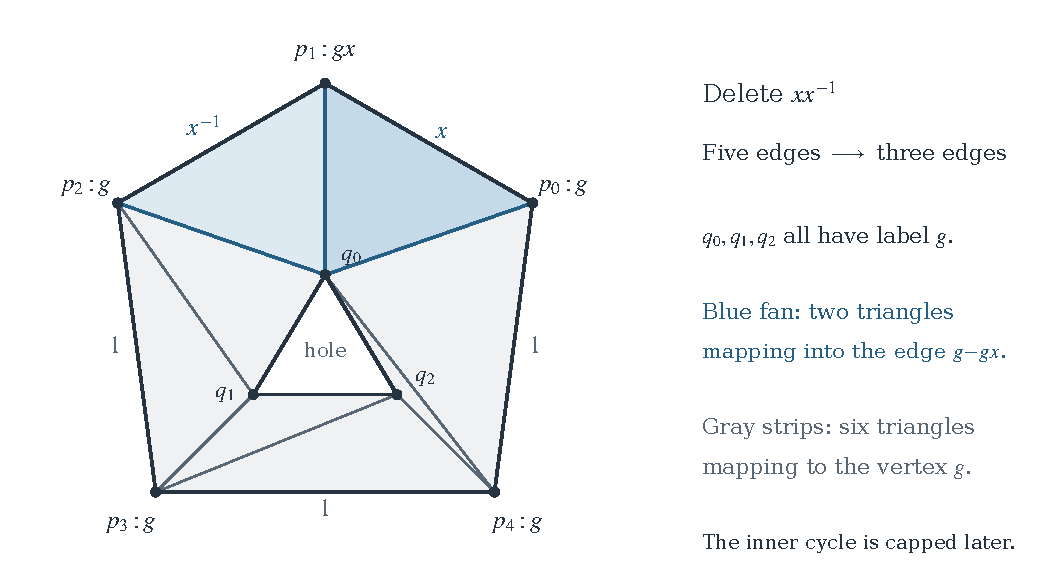
\includegraphics[width=.95\textwidth]{figures/annulus.pdf}
 \caption{The annulus deleting \(xx^{-1}\) and retaining three
 constant steps.  The five outer labels are \(g,gx,g,g,g\);
 the three inner labels are all \(g\).
 The two fan triangles map into the edge from \(g\) to \(gx\);
 the six triangles in the other three strips map to \(g\).
 The inner boundary is capped only at the end of the reduction.}
 \label{fig:annulus}
\end{figure}

Stack the finitely many annuli and cap the final three-step
constant cycle by a cone mapping to its vertex.  The result
is a finite triangulated disk with the original subdivided
boundary.  Identify this parameter disk with the original
face by a boundary-preserving homeomorphism.  Such an
identification is elementary: realize the stacked annuli
as successive collars inside a disk and the final cone as
its central disk; a prescribed parametrization of the
outer circle extends radially.  The triangulation and its affine
simplex maps are understood in these abstract triangle coordinates; the homeomorphism need not be
affine in any pre-existing coordinates on the parameter surface.
All added triangles are therefore contained in the original face.
Gluing these constructions along the already agreed edge subdivisions
gives a triangulated sphere and preserves $B$ as a subcomplex.

\smallskip\noindent\textit{The uniform estimate.}
It remains to verify the uniform estimate at every parameter
point.  Fix all the above fillings for the finite set of
boundary types.  Normalize their original base vertex to
$1\in T$, and let $L$ be the largest original word length
$d_T(1,s)$ of any vertex label appearing in any one of these
fillings.  This number is finite, including for private
generators in the triangular presentation, since they are
words in $a,b,c$.  It is chosen once and does not depend on
$f$.  In a translated filling based at an original vertex
$v_0$ labelled $s_0$, every label $s$ satisfies
$d_T(s_0,s)\le L$.  Every point $p$ of that original face
then satisfies
\[
\begin{split}
 d_Y(sy,f(p))
 &\le d_Y(sy,s_0y)+d_Y(s_0y,f(v_0))
          +d_Y(f(v_0),f(p))\\
 &\le DL+R+1.
\end{split}
\]
Each final triangle lies within that face, so taking
$C_1=DL+R+1$ proves \eqref{eq:all-points-control}.
\end{proof}
